The \ATLAS\ experiment is a general-purpose particle physics detector designed to observe particles produced in the high-energy pp and heavy-ion LHC collisions.
It has a forward–backward symmetric cylindrical geometry and almost $4\pi$ coverage in solid angle.
\ATLAS\ uses a right-handed coordinate system with its origin at the nominal interaction point (IP) in the center of the detector and the z-axis running along the beam line.
The x-y plane is perpendicular to the beam line, and is referred to as the transverse plane.
The x-axis points from the IP to the center of the LHC ring, and the y-axis points upward toward the earth's surface.
The detector half at positive z-values is referred to as the ``A-side'', the other half the ``C-side''.
Cylindrical coordinates (r, $\phi$) are used in the transverse plane, $\phi$ being the azimuthal angle around the beam pipe.
The polar angle $\theta$ is defined as the angle from the positive z-axis. The polar angle is often reported in terms of pseudorapidity, defined as $\eta = -\ln[\tan(\frac{\theta}{2})]$.
The inner tracking detector (ID) used for charged-particle tracking covers the pseudorapidity range $|\eta|<$  2.5 and consists of a silicon pixel detector, a silicon microstrip detector (SCT), and a transition radiation tracker (TRT) in the range $|\eta|<$ 2.0. 
The ID is immersed in a 2 Tesla axial magnetic field produced by a thin superconducting solenoid.
Electromagnetic (EM) and hadronic calorimeters outside the solenoid cover the pseudorapidity range $|\eta|\leq 3.2$.
A 4 Tesla toroid magnet then surrounds the calorimeters.
Interleaved and surrounding the toroid barrel and endap magnets are the muon spectrometers, covering $|\eta|\leq 2.7$.
\begin{figure}[h]
  \begin{center}
    %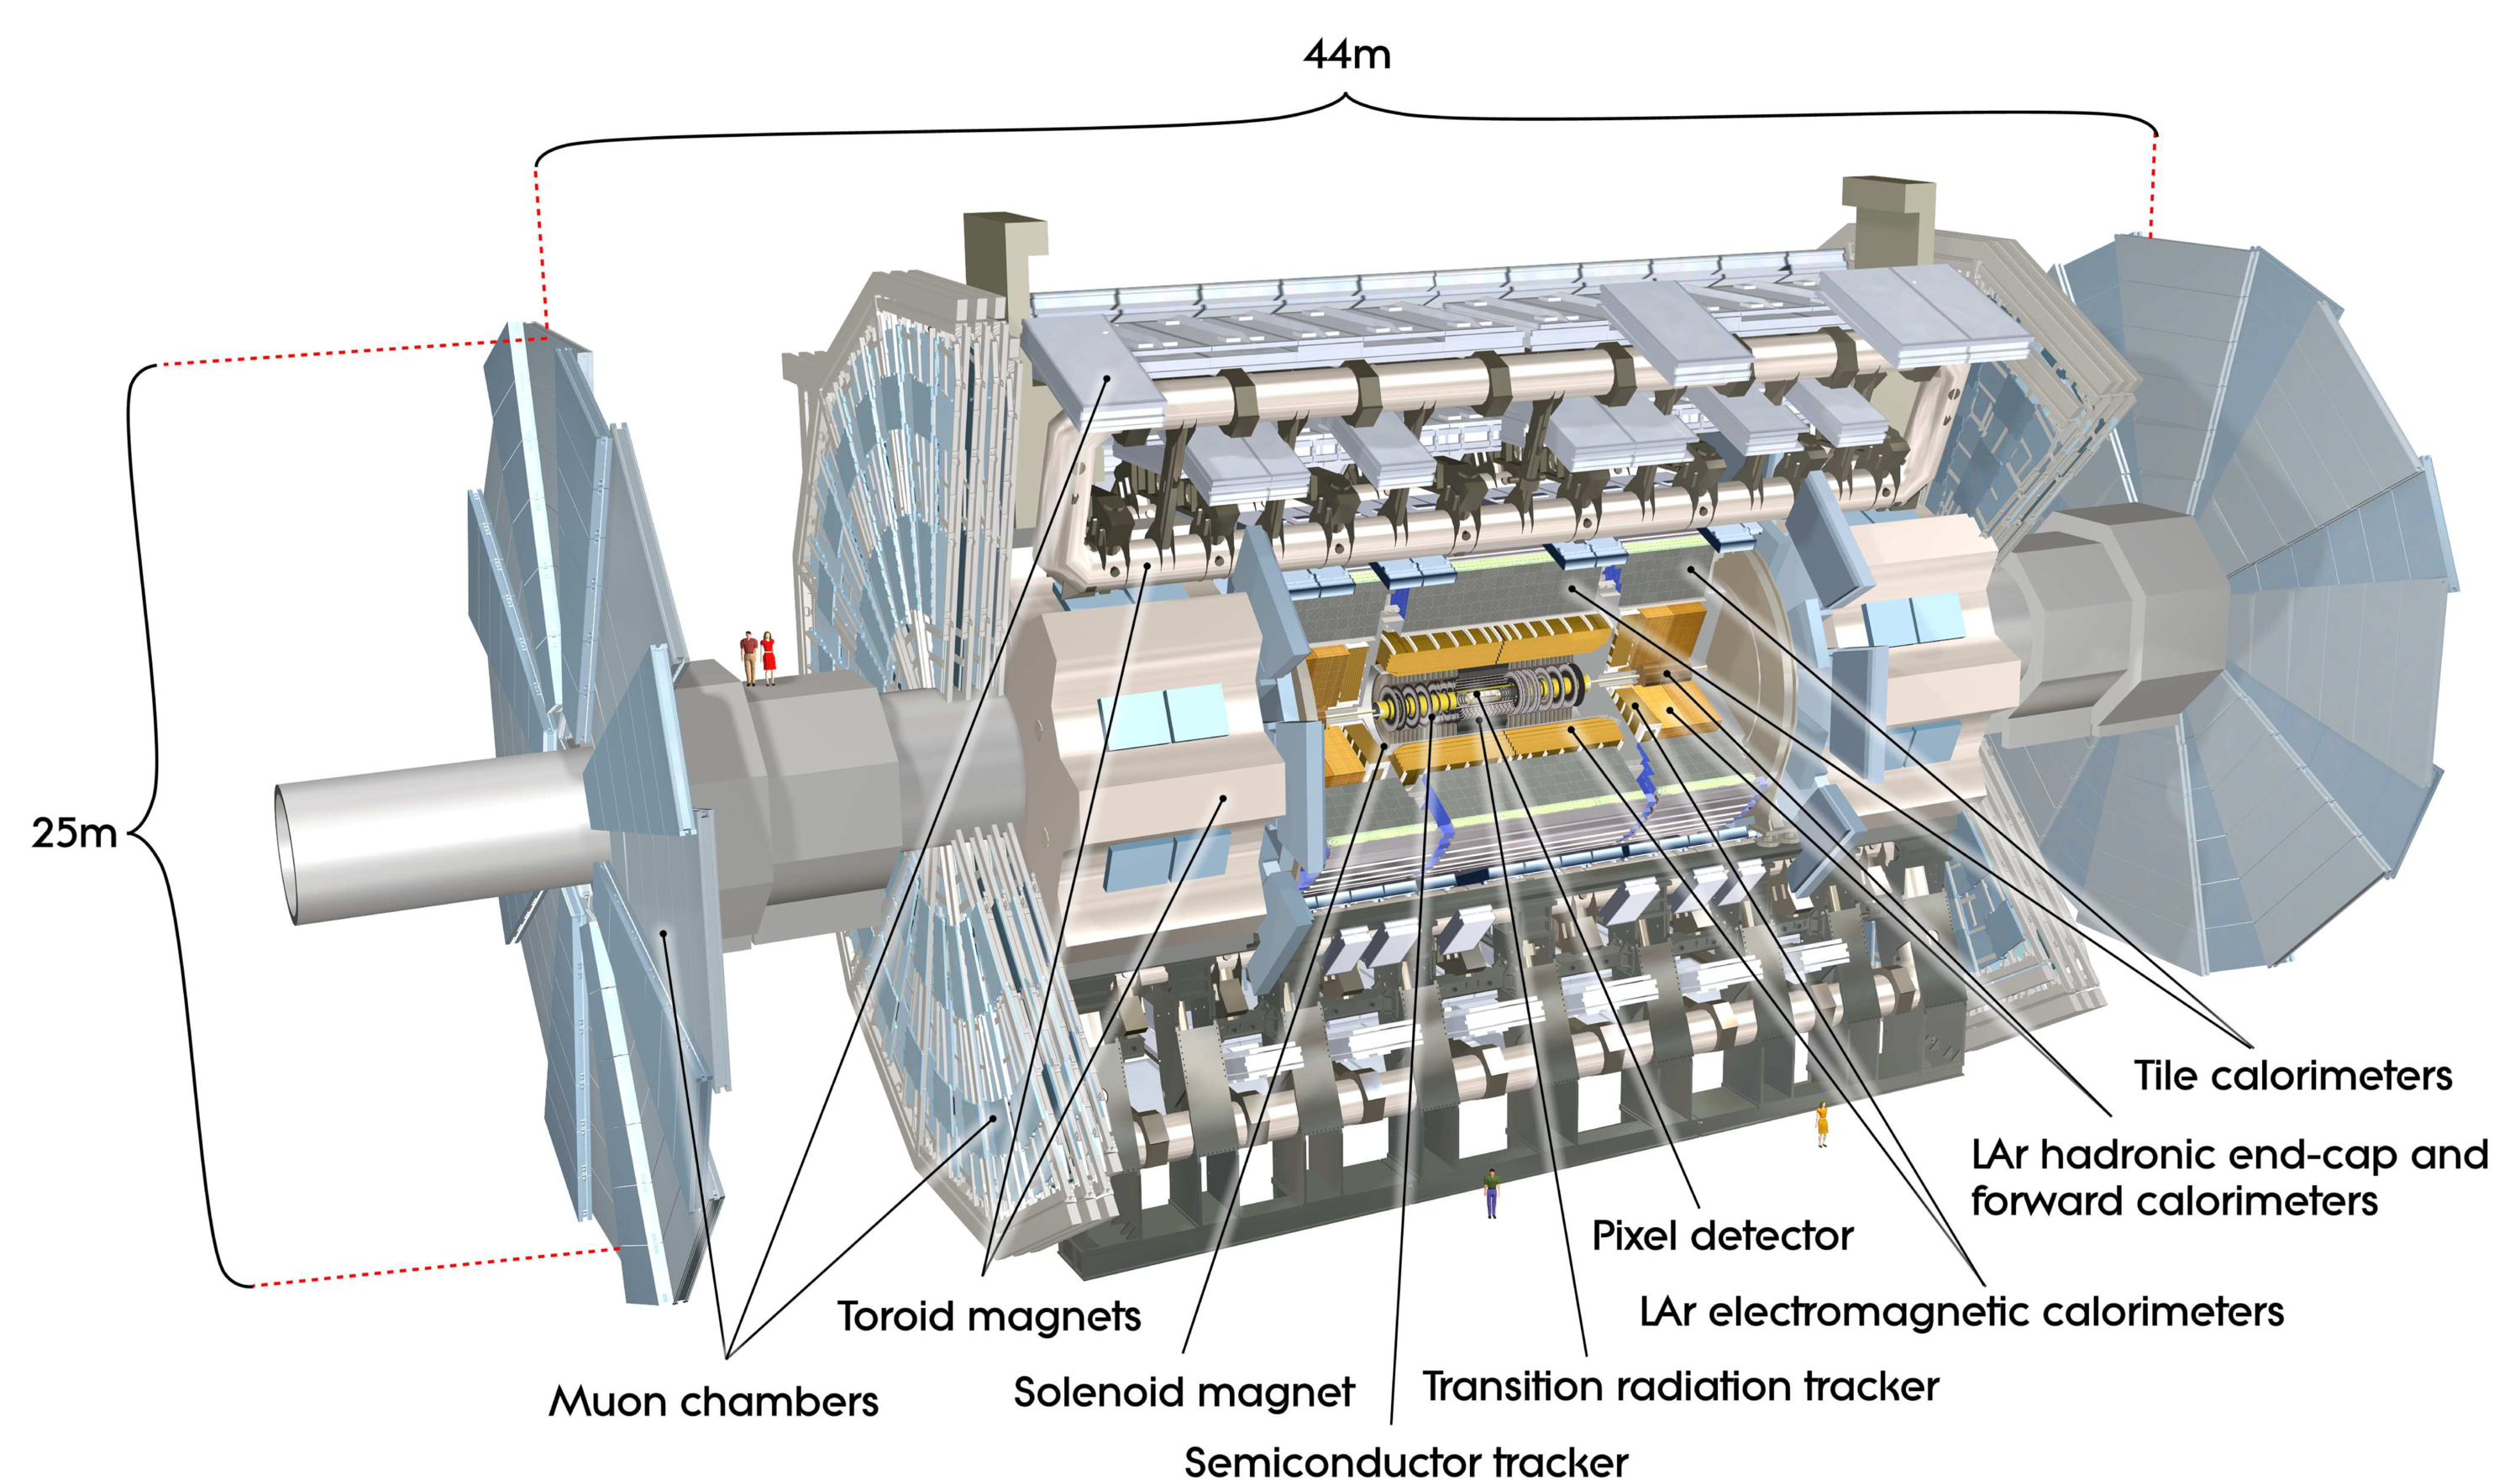
\includegraphics[width=0.3\textwidth]{figs/detector/atlas.png}
    \makebox[\textwidth][c]{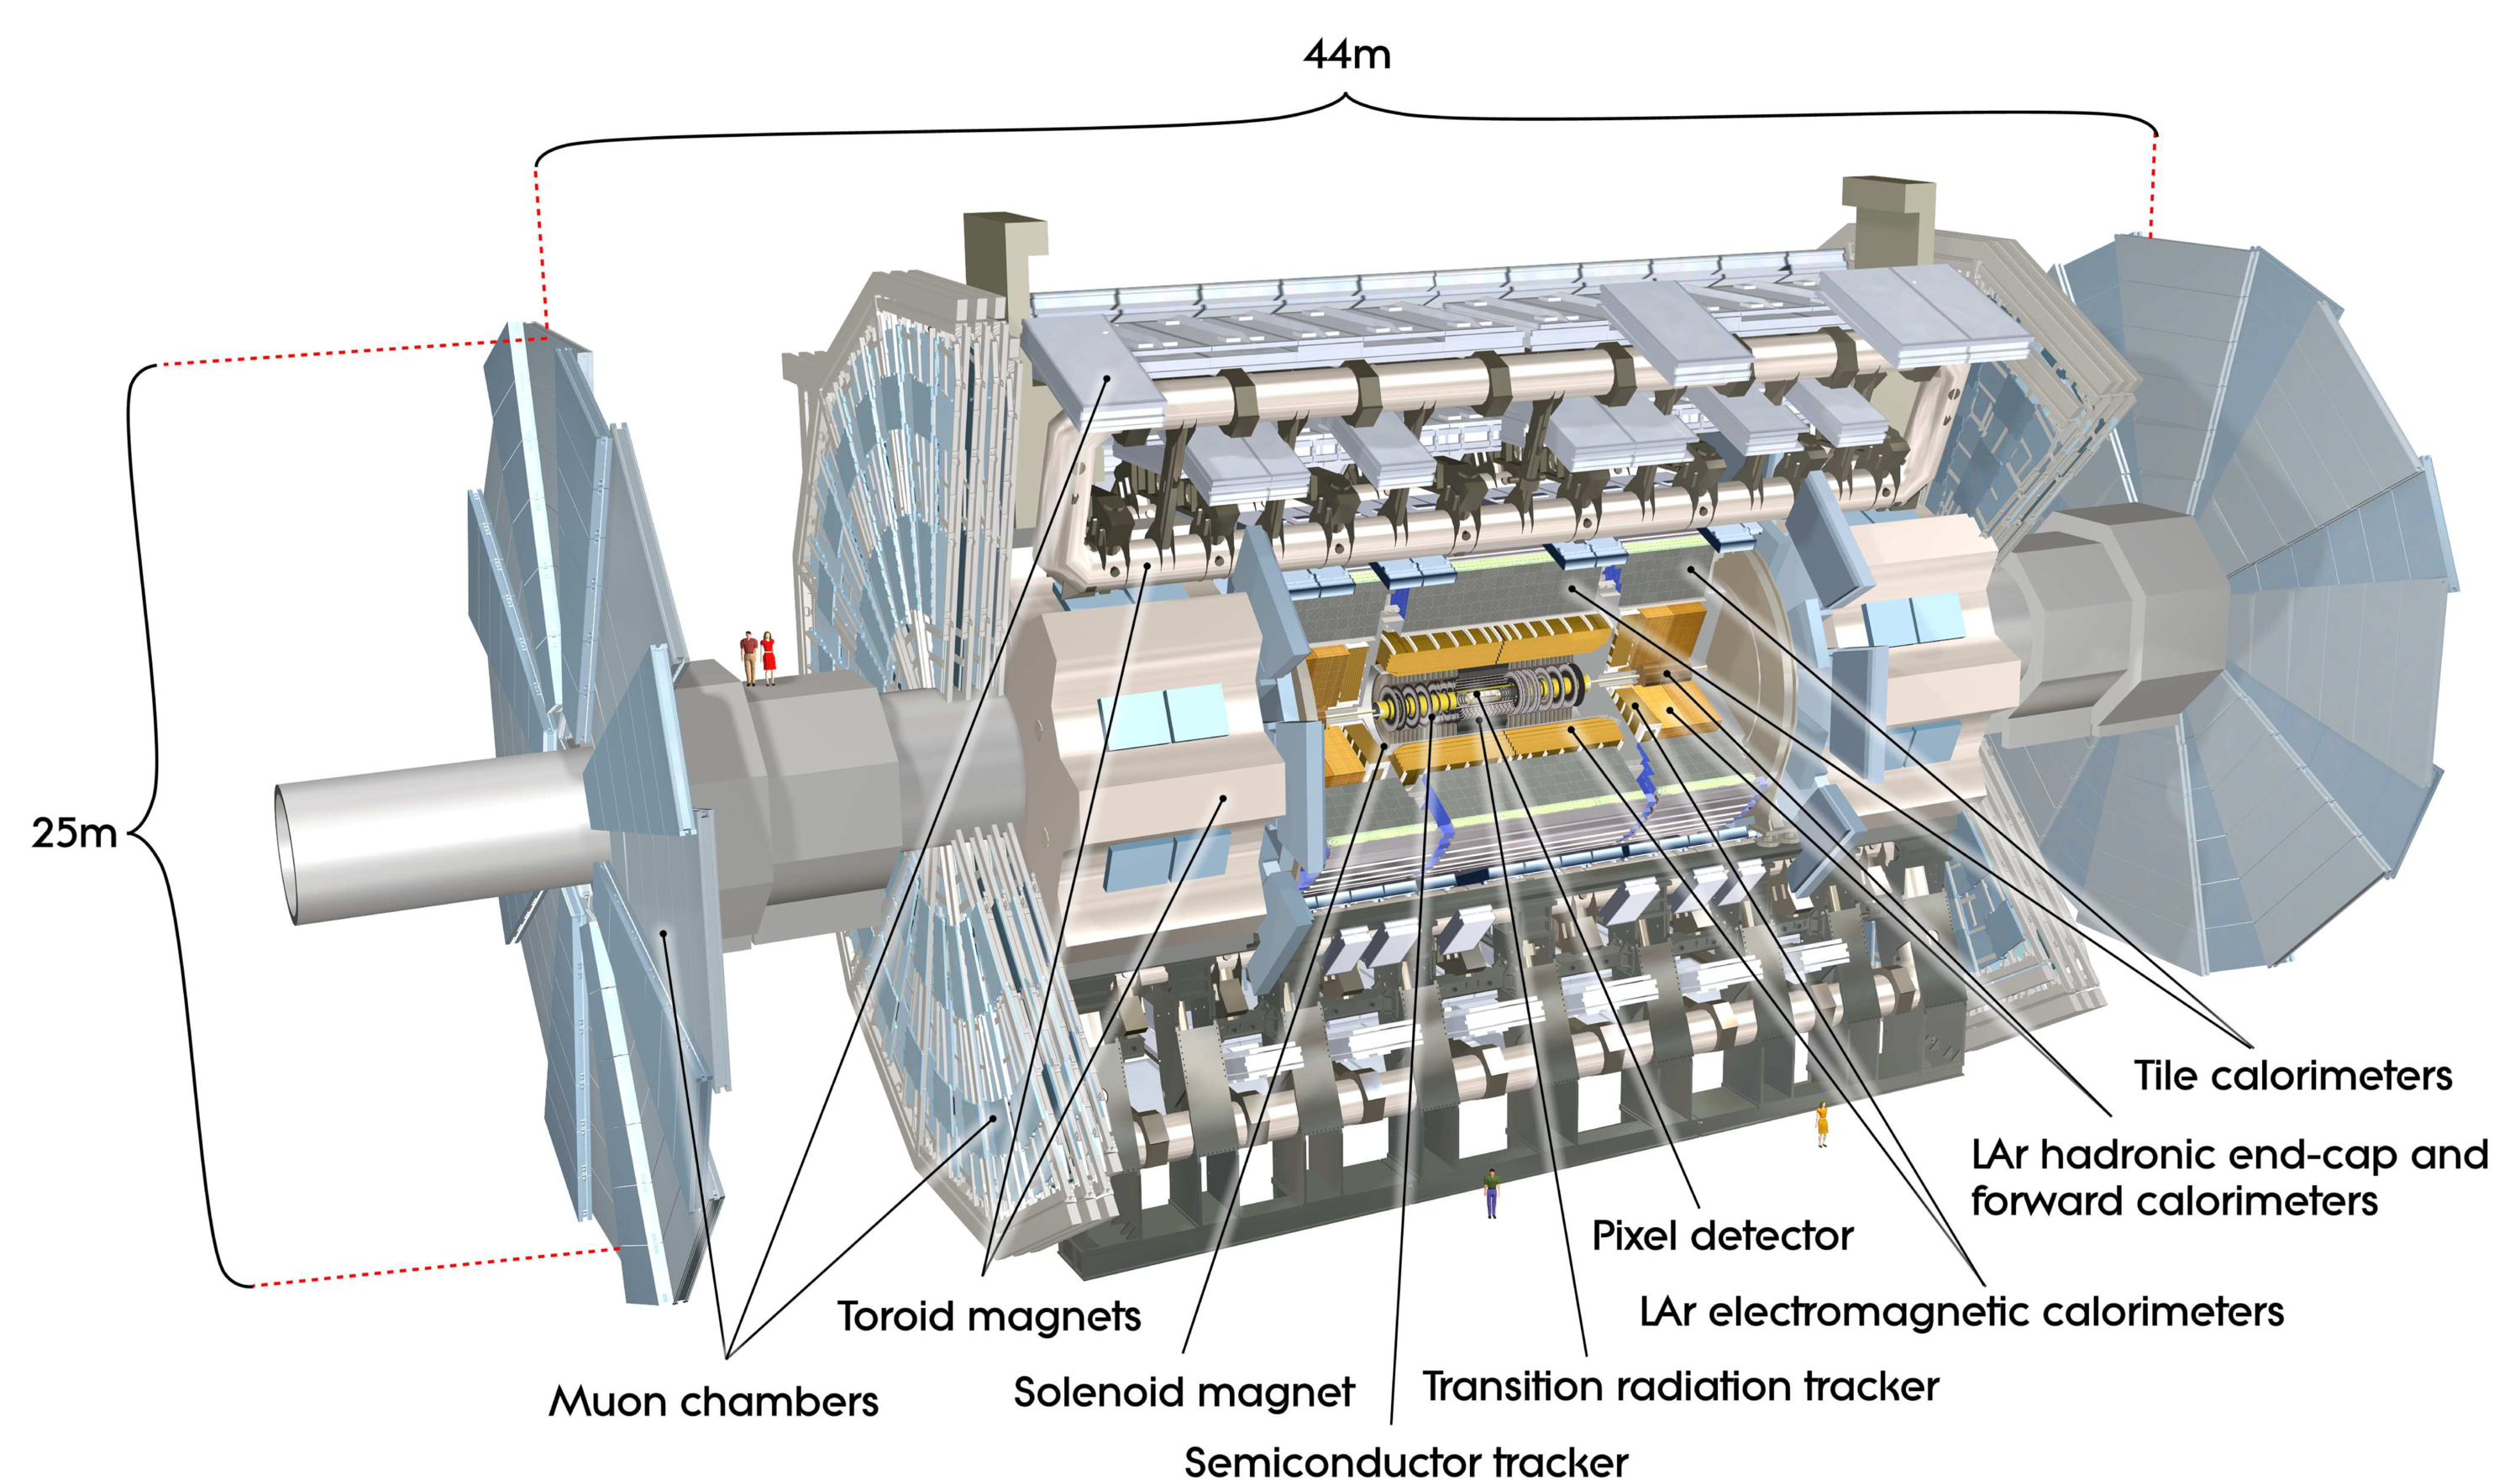
\includegraphics[width=1.24\textwidth]{figs/detector/atlas.png}}
  \end{center}
  \caption[General cut-away view of the ATLAS detector.]
          {General cut-away view of the ATLAS detector \cite{PERF-2007-01}.}
  \label{fig:detector:ATLAS}
\end{figure}
A two-level triggering system reduces the total data-taking rate to approximately 1 kHz from the bunch crossing rate of 40,000 kHz.